\documentclass[dvipsnames,12pt]{book}

%Hey, if you're using this preamble it means that it was probably written by Stefano Graziosi (me). If you see something that doesn't make sense, feel free to email me at stefano.graziosi@studbocconi.it
%p.s. in case it's not already evident from the preamble, I'm not a professional LaTeX user, so I'm sure there are better ways to do things. I'm just trying to make it work.

%------------------------------------------------------------------------------
%           LAST UPDATE: 06-01-2025
%------------------------------------------------------------------------------

%I don't own copyright on anything, I just literally copied and pasted together a bunch of stuff.

%Credit goes to the original authors.

%------------------------------------------------------------------------------
%           Packages
%------------------------------------------------------------------------------

\usepackage[all]{xy}
\usepackage{tcolorbox}
\usepackage{graphicx}
\usepackage{hyperref}
\usepackage{xcolor}    
\usepackage{wrapfig}
\usepackage{amsmath, amssymb, amsthm}
\usepackage{titlesec}
\usepackage{halloweenmath}
\usepackage{enumitem}
\usepackage{listings}

\usepackage{titlepic}
\usepackage{pdfpages}

%------------------------------------------------------------------------------
%           Geometry
%------------------------------------------------------------------------------

\usepackage[a4paper,margin=1in]{geometry}
%\usepackage[margin=1in]{geometry}


%------------------------------------------------------------------------------
%           Colours
%------------------------------------------------------------------------------



%------------------------------------------------------------------------------
%           Environments
%------------------------------------------------------------------------------

%Standard \latex box

\newtcolorbox{mybox}[3][]
{
  colframe = #2!25,
  colback  = #2!10,
  coltitle = #2!20!black,  
  title    = {#3},
  #1,
}

%Standard "Problem" environment

\newtheorem{problem}{Problem}

%Personalised "Solution" environment

\newenvironment{solution}[1][\it{Solution}]{\textbf{#1. } }{$\square$}

%------------------------------------------------------------------------------
%           Code Listing Environment
%------------------------------------------------------------------------------

\lstdefinestyle{mystyle}{
    backgroundcolor=\color{backcolour},   
    commentstyle=\color{codegreen},
    keywordstyle=\color{magenta},
    numberstyle=\tiny\color{codegray},
    stringstyle=\color{codepurple},
    basicstyle=\ttfamily\footnotesize,
    breakatwhitespace=false,         
    breaklines=true,                 
    captionpos=b,                    
    keepspaces=true,                 
    numbers=left,                    
    numbersep=5pt,                  
    showspaces=false,                
    showstringspaces=false,
    showtabs=false,                  
    tabsize=2
}

\lstset{style=mystyle}

\graphicspath{ {./images/} }

\titlepic{
    \makebox[0pt][c]{\hspace*{0.135cm}%
    
\includegraphics[width=\paperwidth]{20236 Logo.png}
    }
}
\title{20236 Time Series Analysis \\[1cm] \textbf{Lecture Notes}}
\author{Stefano Graziosi, Università Bocconi}
\date{\today}

\begin{document}

\maketitle

\tableofcontents

\chapter*{Introduction}

    \section*{Group Project}

        The project will be about climate, taking inspiration from the Bocconi summer school (with two famous experts in climate).

        \noindent Data will be posted fully by week 2.

        

\part{Descriptive techniques and forecasting algorithms}

    \chapter{Classical time series decomposition}

            \section{What is a time series?}

                \begin{mybox}{BlueGreen}{\textbf{Reference}}
                    Chatfield, Ch 2, Sections 2.1-2.6. Subsection 2.5.2: only basic moving average. Section 2.7 will be useful later
                \end{mybox}

                A first answer: a sequence of observations taken over time.
                \begin{equation}
                    y_{1:t} = (y_1, \ldots, y_t)
                \end{equation}

                \begin{figure}[h]
                    \centering
                    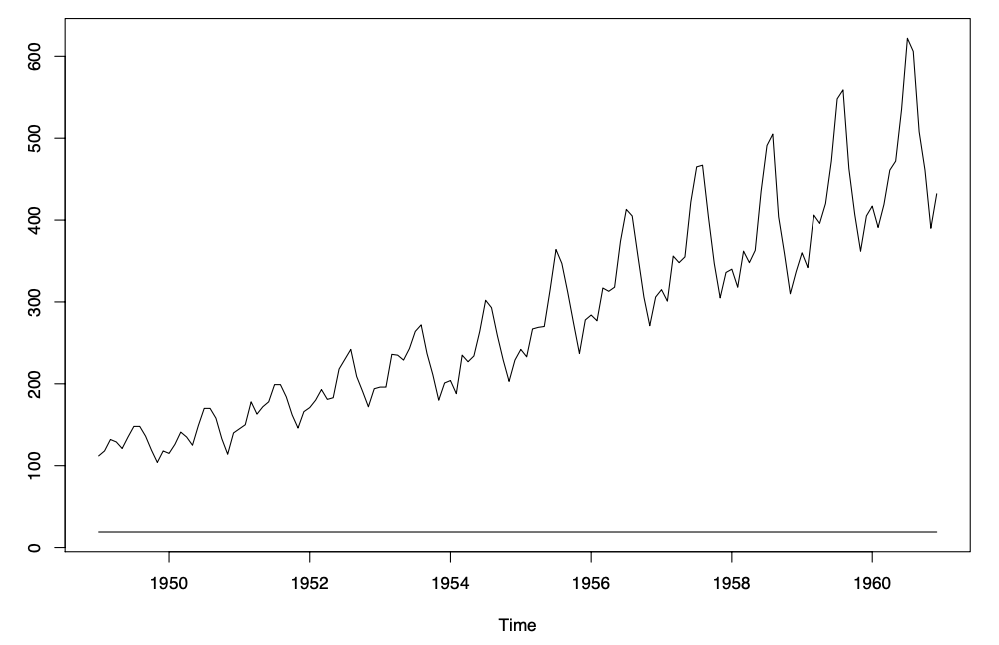
\includegraphics[width=0.48\linewidth]{L1-1.png}
                    \caption{Time plot}
                    \label{fig:L1-1}
                \end{figure}

                The time points of measurement can be:

                \begin{itemize}
                    \item Regularly spaced\footnote{(monthly, yearly, weekly)}, with \textbf{no} missing values \(\rightarrow\) \textbf{discrete time}
                    \item Regularly spaced, with missing values
                    \item Irregularly spaced
                    \item High frequency \(\rightarrow\) \textbf{continuous time}
                \end{itemize}

            \begin{minipage}{0.48\textwidth}
                \textbf{Discrete time}

                    \begin{equation}
                        y_t,t = 1,2,3, \ldots , T
                    \end{equation}
                    
            \end{minipage}
            \begin{minipage}{0.04\textwidth}
                \hfill\vline\hfill
            \end{minipage}
            \begin{minipage}{0.48\textwidth}
                \textbf{Continuous time}

                    \begin{equation}
                        y_t,t \in (1,T)
                    \end{equation}
            \end{minipage}

            \subsection{Different Types of Data}

                \begin{itemize}
                    \item \textbf{Types of data by nature}
                        \begin{itemize}
                            \item Categorical
                            \item Discrete
                            \item Continuous
                        \end{itemize}
                    \item \textbf{Types of data by dimensionality}
                        \begin{itemize}
                            \item Univariate
                            \item Multivariate
                        \end{itemize}
                \end{itemize}

            \subsection{Aims of time series analysis}

                \begin{enumerate}
                    \item \textbf{Exploratory/descriptive analysis}
    
                        Describe trend, seasonality, cycle, etc. 
                        Often, in order to de-trend, de-seasonalize, etc.
                        Multivariate/high dimensional time series: summarize; find common patterns, clusters, dimension reduction, etc...
                        
                    \item \textbf{Forecasting}
    
                        There are clever algorithms for forecasting (a first example: simple exponential smoothing).
                        \textbf{Issue:} they do not describe \textit{uncertainty} and \textit{risk}, nor give a ‘\textit{vision}’ of the phenomenon (long tern forecasts).
                    
                    \item \textbf{Explain}
    
                        In fact, we may want to explain the phenomenon; understand the relationships among variables, or how one variable of interest Y depends on other variables. These will not be determinist relationships, but ‘statistical ’. The main tool is regression! But, here, the variables evolve over time.
    
                    \item \textbf{Modelling and inference}
    
                        In this "explain" task, the info on the phenomenon is formalized through a \textbf{probabilistic (statistical) model}. The statistical model will have unknown parameters, that will have to be estimated: \textbf{inference}\footnote{Statistical inference is based on probability.}.
    
                    \item \textbf{Forecasting \(\Rightarrow\) Decisions under Risk}
    
                        Still, the ultimate goal is \textbf{forecasting}: but now we have probability to express uncertainty and risk.
                        
                \end{enumerate}
    
                \paragraph{What is a time series?}
    
                    In this all, a time series is no longer just a sequence of measurements over time, but a stochastic process \(Y_t, t \geq 1\).
    
                    In the course we will study some of the main probabilistic models for time series analysis, with focus on models for non-stationary processes.

\newpage

                \begin{remark}
                    \textbf{Aims of time series analysis}
                    \begin{enumerate}
                        \item Exploratory/descriptive analysis
                        \item Explain (modelling and inference)
                        \item Forecasting
                        \item Control \(\rightarrow\) One wants to forecast \(y_t\) , but also control \(y_{t+1}\) through control variables \(x_t\)
                        \item Decisions under risk
                    \end{enumerate}
                \end{remark}


        \section{Exploratory analysis}

            \subsection{Classical time series decomposition}
            
                Classical time series decomposition describes a univariate time series \( (Y_t)_{t \geq 1} \) as composed by structural components such as a trend, a seasonal component, a cycle,\dots, and an erratic component
                
                \begin{align}
                    Y_t & = T_t + S_t + C_t + E_t \quad \text{additive} \label{1.4eq} \\
                    Y_t & = T_t * S_t * C_t * E_t \quad \text{multiplicative} \label{1.5eq}
                \end{align}
                
                \noindent Notice that a \textit{log} transforms a multiplicative decomposition into an additive one, for example \ref{1.5eq} becomes:
                
                \begin{equation}
                    \log Y_t = \log T_t + \log S_t + \log E_t
                \end{equation}

            \subsection{Additive seasonality and trend}

                If in \texttt{R} we write:
            
\begin{lstlisting}[language=R]
plot(co2)
\end{lstlisting}

                \noindent We get the following output:

                \begin{figure}[h]
                    \centering
                    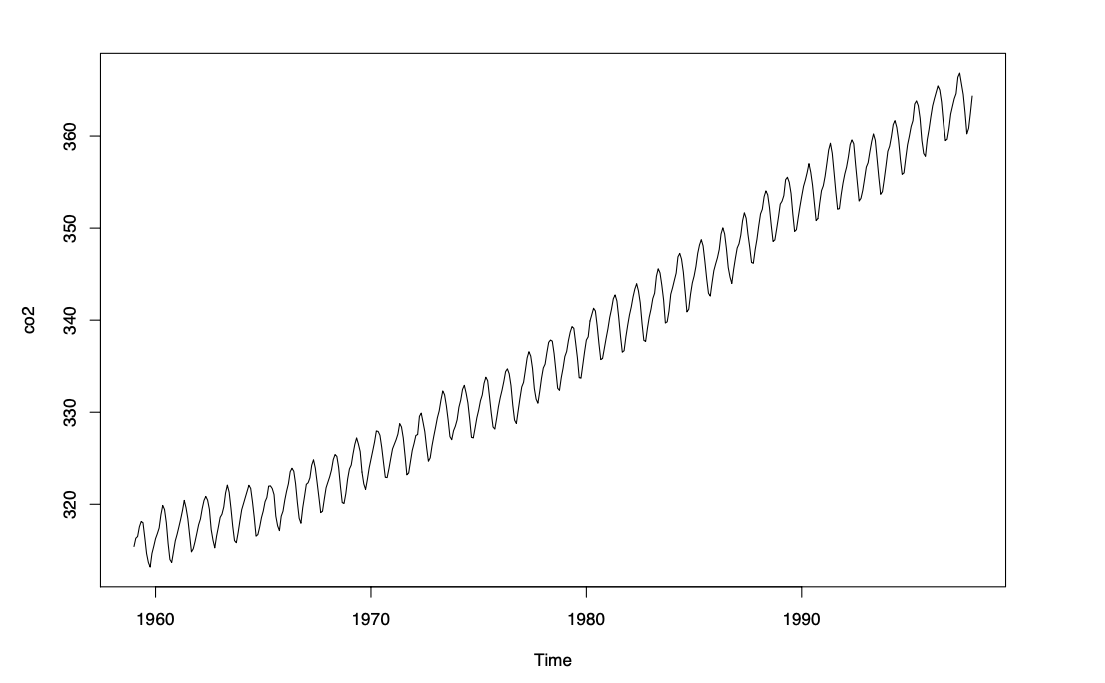
\includegraphics[width=0.5\linewidth]{L1-2.png}
                    \caption{Evolution of CO2 concentration levels}
                    \label{fig:L1-2}
                \end{figure}

\newpage
                \noindent If instead we write:

\begin{lstlisting}[language=R]
plot(AirPassengers)
\end{lstlisting}

                \noindent We get the following output;

                \begin{figure}[h]
                    \centering
                    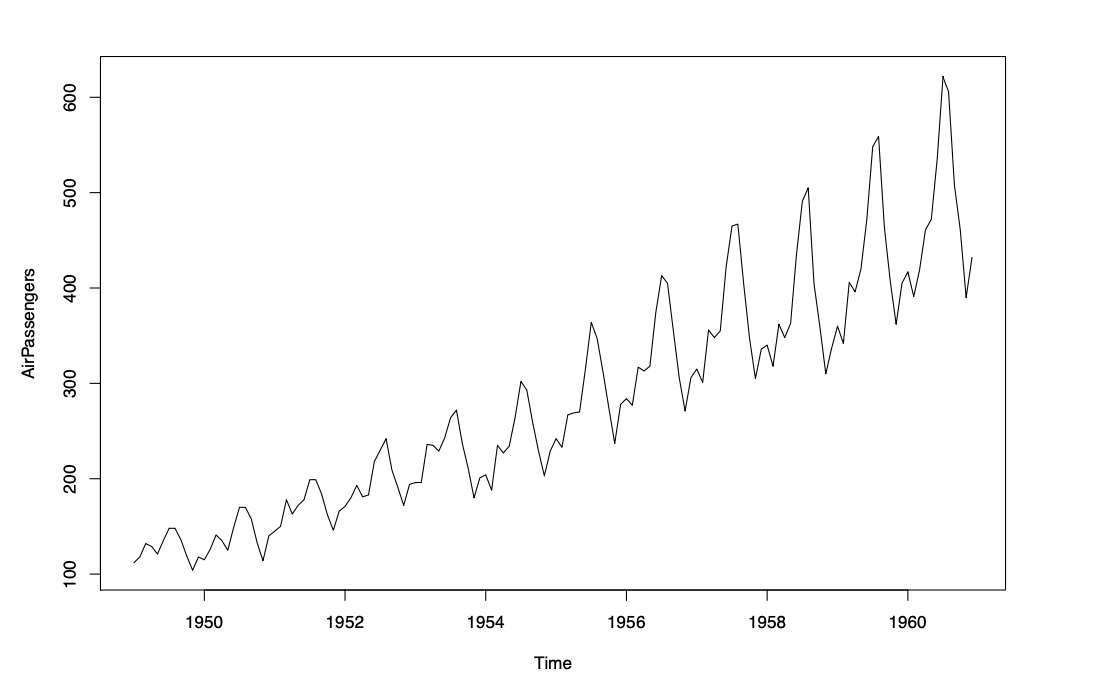
\includegraphics[width=0.5\linewidth]{L1-3.png}
                    \caption{Evolution of air passenger travel}
                    \label{fig:L1-3}
                \end{figure}

            \section{Fitting a trend}

                Consider a series that only shows a trend (no seasonal component)
                \[
                Y_t = T_t + E_t
                \]
                \noindent How can we fit the trend? Main basic tools:

                \begin{enumerate}
                    \item \textbf{Fit a smooth function of \(t\)}

                        For example, take a linear trend:
                        \[
                        y_t = \beta_0 + \beta_1 t + e_t, \quad t = 1, \dots, n
                        \]
                        
                        \noindent Estimate \( \beta_0 \) and \( \beta_1 \) by least squares:
                        
                        \begin{equation}
                            \arg\min_{(\beta_0, \beta_1)} \sum_{t=1}^{n} (y_t - (\beta_0 + \beta_1 t))^2
                        \end{equation}
                        
                        \noindent One can use more complex functions, for example a quadratic trend
                        
                        \begin{equation}
                            y_t = \beta_0 + \beta_1 t + \beta_2 t^2 + e_t
                        \end{equation}
                        
                        \noindent or an exponential trend etc.
                        
                        \begin{remark}
                            But, being too flexible makes it difficult to identify a trend and a cycle
                        \end{remark}

\newpage

                    \item \textbf{Fitting a moving average}

                        For example, a moving average of order \( k = 3 \):

                        \begin{equation}
                            \hat{T}_t = \frac{y_{t-1} + y_t + y_{t+1}}{3}, \quad t = 2,3,\dots
                        \end{equation}
                        
                        \noindent gives a ‘smoothed version’ (\(\hat{T}_t\)) of the observed series, interpreted as the trend; the higher \( k \), the smoother the fitted trend.
                        
                        \noindent If \( k \) is even, e.g. \( k = 4 \), use
                        
                        \begin{equation}
                            \hat{T}_t = \frac{0.5 y_{t-2} + y_{t-1} + y_t + y_{t+1} + 0.5 y_{t+2}}{4}
                        \end{equation}

                        Having fitted the trend \( \hat{T}_t \), let

                        \[
                        y_t = \hat{T}_t + E_t, \quad t = 2, \dots, n
                        \]
                        
                        We can remove the trend, to obtain a \textit{de-trended} time series
                        
                        \begin{equation}
                            y_t^{\text{detrended}} = y_t - \hat{T}_t
                        \end{equation}
                \end{enumerate}

            \section{Fitting a seasonal component}

                Consider a purely seasonal time series (no trend).
                
                \begin{equation}
                    Y_t = S_t + E_t
                \end{equation}

                How can we fit the seasonal component? Main basic tools:

                \begin{enumerate}
                    \item \textbf{Seasonal factors}

                        Suppose you have monthly data \( y_t \), with mean \( \bar{y}_t = 0 \). A simple way to proceed is to introduce \textit{seasonal factors}  \( \alpha_{Jan}, \alpha_{Feb}, \dots, \alpha_{Dec} \) and describe
                        
                        \begin{equation}
                            y_t = \alpha_{\text{month}(t)} + E_t
                        \end{equation}
                        
                        where, if \( t \) corresponds to January, \( \alpha_{\text{month}(t)} = \alpha_{Jan} \), and so on. 
                        
                        \noindent For identifiability, we assume that the sum of the seasonal factors is zero. (Remember we are only considering additive decomposition.)

                    \item \textbf{Moving averages}

                        For example, with monthly data, use MA(12)

                        \begin{equation}
                            y_t^{\text{deseasonalized}} = \frac{0.5 y_{t-6} + y_{t-5} + \dots + y_{t+5} + 0.5 y_{t+6}}{12}
                        \end{equation}
                \end{enumerate}

\newpage
                
        \section{Fitting trend and seasonal components}

            Now consider

                \begin{equation}
                    T_t + S_t + E_t
                \end{equation}

            \begin{enumerate}
                \item \textbf{Detrend, then fit the seasonal component}

                    e.g., the R function \texttt{DECOMPOSE} uses MA to fit the trend \( \hat{T}_t \) and, on the detrended series

                    \begin{equation}
                        y_t^{\text{detrended}} = y_t - \hat{T}_t
                    \end{equation}

                    estimates the seasonal factors;

                \item \textbf{Fit the seasonal component, then detrend}

                    Fit the seasonal component, and on the deseasonalized series, fit the trend.

            \end{enumerate}

\begin{lstlisting}[language=R]
    plot (co2)
\end{lstlisting}

            \begin{figure}[ht]
                \centering
                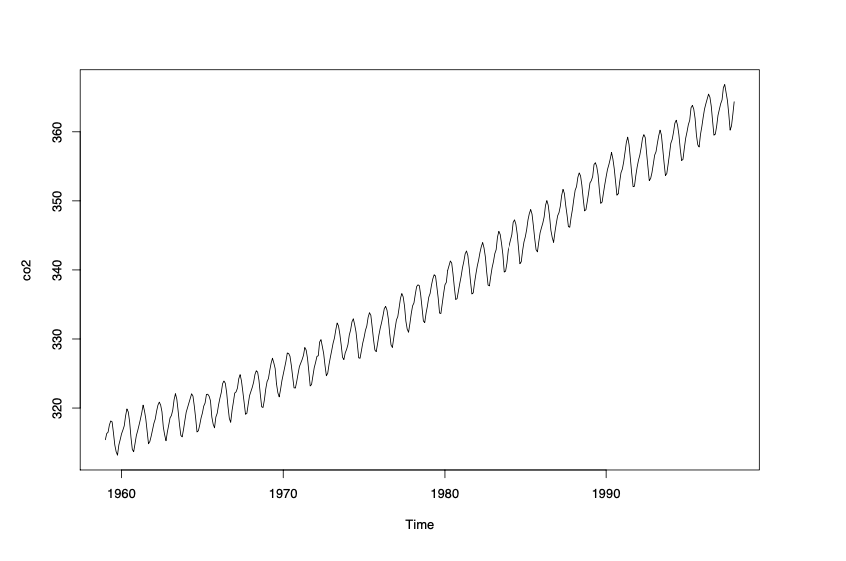
\includegraphics[width=0.5\linewidth]{L1-4.png}
                \caption{Atmospheric concentrations of CO2 are expressed in parts per million (ppm) and reported in the preliminary 1997 SIO manometric mole fraction scale. Monthly data from 1959 to 1997.}
                \label{fig:L1-4}
            \end{figure}

            \begin{example}
                In Laboratory 1 we’ll introduce time series analysis with R and use R functions for time series decomposition.
            \end{example}

%----------------------------------------

    \chapter[Simple exponential smoothing]{Forecasting algorithms: Simple exponential smoothing}
    
        \begin{mybox}{BlueGreen}{\textbf{References}}
            Chatfield (2004), Ch.5, sect. 5.2.2; Petris, Petrone, Campagnoli (2009), Chapter 3, section 3.3.1
        \end{mybox}

        \section{Forecasting algorithms}

            Forecasting (and consequent decisions) is often the ultimate goal of time series analysis. 
            
            Forecasting algorithms: predict $y_{t+1}$ given $y_{1:t}$
            
            We present  \textbf{exponential smoothing}, a simple and cleaver algorithm, also called Holt-Winters algorithm, after Holt (1957) and Winters (1960).

        \section{Simple exponential smoothing}

            Consider a time series that shows no trend and no seasonality. At time $t$, we want to provide a forecast of $y_{t+1}$ given data $(y_1, \ldots, y_t)$ (that I will denote by $y_{1:t}$ for short).

            The idea is to take a weighted average of the past values $y_{1:t}$
            
            \begin{equation}
                \hat{y}_{t+1|t} = c_0 y_t + c_1 y_{t-1} + \ldots + c_{t-1} y_1
            \end{equation}

            with geometrically decreasing weights:

            \begin{equation}
                c_j= \alpha (1-\alpha)^j , 0< \alpha < 1
            \end{equation}

            Remembering the geometric series:$\sum_{j=0}^\infty \lambda^j = \frac{1}{1-\lambda}$ if $0 < \lambda < 1$, we have

            \begin{equation}
                \sum_{j=0}^\infty \alpha (1-\alpha)^j = \alpha \sum_{j=0}^\infty  (1-\alpha)^j = \alpha \; \frac{1}{1- (1 - \alpha)} = 1
            \end{equation}

            Thus, if $t$ is large, the weights' sum in the average above is approximately one. \\

            Thus, the \textit{simple exponential smoothing algorithm} gives the point forecast:

            \begin{equation}
                \hat{y}_{t+1|t} = \alpha y_t + \alpha (1-\alpha) y_{t-1} + \alpha (1-\alpha)^2 \ldots +  \alpha (1-\alpha)^{t-1} y_1
            \end{equation}

        \section{Recursive form}

            \begin{align}
                \hat{y}_{t+1 | t} = & \ \alpha y_t + (1-\alpha) \, [\alpha  y_{t-1} + \alpha (1-\alpha) \ldots +  \alpha (1-\alpha)^{t-2} y_1] \\
                = & \ \alpha y_t + (1-\alpha) \hat{y}_{t | t-1}
            \end{align} 

            \begin{remark}
                \begin{itemize}
                    \item if $\alpha \approx 1$,  $\hat{y}_{t+1|t} \approx y_t$ 
                    \item if $\alpha \approx 0$,  $\hat{y}_{t+1|t} \approx constant$
                \end{itemize}
            \end{remark}

            \begin{definition}
                The parameter $\alpha$ is called \textbf{smoothing parameter}
            \end{definition}

            \subsection{Error correction form}
    
                \begin{equation}
                    \hat{y}_{t+1 | t} = \hat{y}_{t | t-1} + \alpha \underbrace{(y_t - \hat{y}_{t | t-1})}_{\text{Forecast error}}
                \end{equation}
    
                \begin{itemize}
                    \item at time $t-1$, forecast $\hat{y}_{t | t-1}$
                    \item then observe $y_t$
                    \item and correct the forecast, taking into account the forecast error
                \end{itemize}

            \subsection{Choosing \(\alpha\)}

                Algorithms have parameters that need to be "tuned" (on a training sample). Here, we have to tune the smoothing parameter $\alpha$: 

                \begin{itemize}
                    \item consider a (fine) grid of values of $\alpha$ in $(0,1)$
                    \item for each $\alpha$, use the algorithm to recursively compute the one-step-ahead forecasts, for $t=1, \ldots, T$
                    \item "Score" the forecasts and choose the value $\alpha$ that gives the best predictive performance. 
                \end{itemize}

            \subsection{Popular measures of predictive performance}

                $e_t = y_t - \hat{y}_{t | t-1}$   \textbf{forecast error}

                \begin{equation}
                    MAE= \frac{\sum_{t=1}^T | e_t |}{T}  \quad \quad \mbox{Mean Absolute Value}
                \end{equation}

                \begin{equation}
                    MSE =  \frac{\sum_{t=1}^t | e_t^2 |}{T}  \quad \quad \mbox{Mean Square Error}
                \end{equation}

                \begin{equation}
                    MAPE =  \frac{\sum_{t=1}^T | \frac{e_t}{y_t} |}{T}  \quad \quad \mbox{Mean  Absolute Percentage Value}
                \end{equation}

                Note that the latter measure does not depend on the scale.

            \subsection{Extensions}

                Simple exponential smoothing does not envisage a trend nor a seasonal behaviour. The so-called \textit{Holt-Winters} forecasting algorithm extends simple exponential smoothing to the case of trend and/or seasonality. 

                \noindent Here we briefly present these extensions; our aim is simply to understand how the \texttt{R} functions for exponential smoothing work.

                \noindent Only simple exponential smoothing is part of the program for the written proof in the final exam; but you may want to use these extension in your data project.

                \begin{remark}
                    We will give a probabilistic interpretation of these algorithms  as Dynamic Linear Models. 
                \end{remark}

        \section{Forecast function}

            We didn't give a definition of "trend". Let's here think of the trend as the "expected" future behaviour of the time series.  

            \begin{definition}
                Define the forecast function

                \begin{equation}
                    f_t : h \rightarrow f_t(h) \equiv \hat{y}_{t+h | t} \; , \quad \quad h=1, 2, \ldots
                \end{equation}
                
            \end{definition}

            In simple exponential smoothing, the forecast function at time $t$ is defined as a constant function of $h$,

            \begin{equation}
                f_t(h) \equiv \hat{y}_{t+h | t} = \hat{y}_{t+1 | t}, \quad h=1, 2, \ldots
            \end{equation}

            Which is a "flat" prediction.

            \subsection{Intuition: $y_t$ only shows a "level"}

                The idea is that 
                $$ y_t = level+ \epsilon_t $$
                and we are forecasting the level; thus a "flat" forecast function seems reasonable.
                
                In fact (as we will explain rigorously through DLMs), the idea is more clever than that, 
                $$ y_t = level_t + \epsilon_t $$
                and we update the forecast of the level as

                \textcolor{red}{$$L_t = \alpha y_t + (1-\alpha) L_{t-1} .$$}

                Denoting \textcolor{red}{$\hat{y}_{t+1 | t} = L_t $} (level forecast, made at time $t$),  thus 
                \textcolor{red}{$\hat{y}_{t | t -1 }= L_{t-1}$} (level forecast, made at time $t-1$),
                we see that the rule above corresponds to the forecast rule we had
                $$ \hat{y}_{t+1 | t} = \alpha \, y_t + (1-\alpha) \hat{y}_{t | t-1}. $$

                \subsubsection{Extension to a trend}

                    Let us now consider a time series that shows a (possibly time-evolving) trend; no seasonal component. 
                    
                    Forecast function:
                    $$ f_t (h) = L_t + B_t \; h, \quad \quad  h=1, 2, \ldots , $$
                      where the forecasts for the level, $L_t$, and for the growth, $B_t$, are recursively updated with a similar rule
                    \textcolor{red}{\begin{eqnarray}
                      L_t &=& \alpha y_t + (1-\alpha) (L_{t-1} + B_{t-1})\\
                      B_t &=& \beta (L_t - L_{t-1}) + (1-\beta) B_{t-1}
                      \end{eqnarray}}
                    where
    
                    \begin{itemize}
                        \item \textcolor{red}{$L_{t-1} + B_{t-1} = \hat{y}_{t | t-1}$}, so the first update is "the same" as in simple exponential smoothing; 
                        \item \textcolor{red}{$(L_t - L_{t-1})$} growth estimate at time $t$ (difference of the levels); 
                        \item \textcolor{red}{0$B_{t-1}$} growth estimate at time $t-1$.
                    \end{itemize}
                
                \subsubsection{Extension to a seasonality}

                    Consider, for example, monthly data 

                    Seasonal factors: (think, e.g., of $t$=January)
                    $$S_t \approx S_{t+ 12} \approx S_{t+ 2* 12} \approx \cdots  $$

                    Similar idea for this forecast function:

                    \begin{equation}
                        \hat{y}_{t+h | t} = L_t + B_t \, h + S_{t+m+h}
                    \end{equation}

                    where 
                    \textcolor{red}{\begin{eqnarray}
                      L_t &=& \alpha (y_t - S_{t-m}) + (1-\alpha) (L_{t-1} + B_{t-1})\\
                      B_t &=& \beta (L_t - L_{t-1}) + (1- \beta) B_{t-1} \\
                      S_t &=& \gamma (y_t - (L_{t-1}+B_{t-1})) + (1-\gamma) S_{t-12}
                      \end{eqnarray}}

                    For now, enough to remember that there are three smoothing parameters, $\alpha$, $\beta$, $\gamma$, referring to level, growth, seasonality

%----------------------------------------        

%    \chapter{Laboratory 1}
%
%        \begin{mybox}{BlueGreen}{}
%        
%            Introduction to time series analysis with R. (Rcode, with commented examples \& data: posted on BlackBoard (BB)).
%            
%            \textbf{Running application}: climate. Dataset, material, questions \& getting started with the final project
%        \end{mybox}
        
%----------------------------------------
%---------------------------------------- 
\part{Probabilistic Models for Time Series Analysis}
%----------------------------------------
%----------------------------------------

    \chapter[Introd. to Probabilistic Models]{Introd. to Probabilistic Models for Time Series Analysis}

        \begin{mybox}{BlueGreen}{\textbf{Further readings:}}
            Chatfield, Chapter 3, Sections 3.1–3.4, and references therein
        \end{mybox}

        \section{Time series as a stochastic process}

            So far, we have been thinking of a time series as a sequence of measurements taken over time, $y_{1:t} = (y_1, y_2, \ldots, y_t)$. We presented simple exponential smoothing as a simple, but quite clever, forecasting algorithm that recursively provides a point forecast $\hat{y}_{t+1\mid t}$ given data $y_{1:t}$. But how reliable are the algorithm's forecasts? In fact, this is quite a timely question that we could also address to the current hype of AI algorithms. 
            
            As a predictive algorithm, simple exponential smoothing does not provide any  measure of the uncertainty associated with the forecasts. But being able to quantify uncertainty, and the implied risk of decisions based on those forecasts,  is in fact crucial.  
            
            There are many ways to express uncertainty. We could express vague claims such as ``we are pretty sure,'' ``I'm not that confident''; but we want to have a more structured methodology. The statistical methodology quantifies uncertainty around estimates and forecasts through \emph{probability}. 
            
            This means, to start with, a different notion of ``time series.'' 

            \begin{definition}[Time series]
                We define a time series as a \emph{stochastic process} $(Y_t)_{t \in T}$, with $Y_t \in \mathcal{Y}$, where the index $t$ refers to time. The data $(y_t)$ are then regarded as a realization of the stochastic process. (I will often use the short notation $(Y_t)$ for $(Y_t)_{t \in T}$.) 
            \end{definition}
            
            \subsection{What is a stochastic process?} 
            
                You might have studied this notion in previous courses in Statistics or Probability. To our aims, let us recall that a stochastic process $(Y_t)_{t \in T}$ is a sequence of random vectors indexed by $t$, with $t$ in a set $T$. If $T$ is countable, for example $t = 1, 2, \ldots,$ we say that $(Y_t)$ is a discrete-time stochastic process. Or we may have continuous-time stochastic processes. 
                
                Classic time series analysis refers to discrete-time processes. The time series is univariate, if $Y_t \in \mathcal{Y} \subseteq \mathbb{R}$, or multivariate, if $Y_t = (Y_{1,t}, \ldots, Y_{m,t})^T$ is a random vector in  $\mathcal{Y} \subseteq \mathbb{R}^p$. Let us focus, in this introduction,  on the univariate case. Then, for any $t$, $Y_t$ is a random variable,  and $y_t$ denotes a realization of $Y_t$. See the beautiful Figure \ref{fig:L3-1} for a simple illustration.

                    \begin{figure}[h]
                        \centering
                        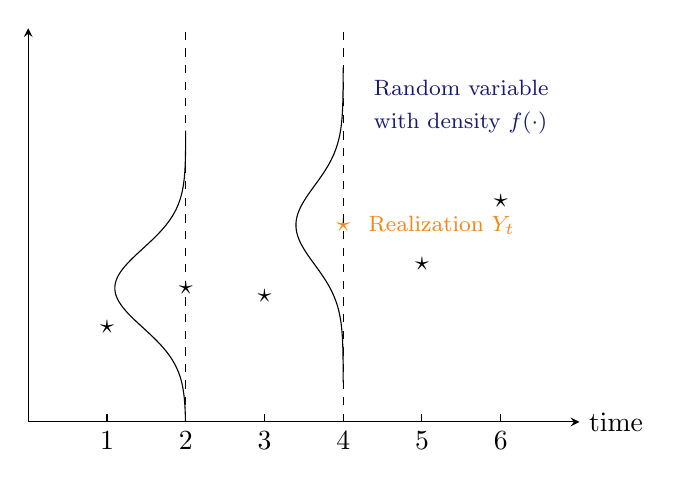
\begin{tikzpicture}[scale=1.0,>=stealth]\label{fig:L3-1}
                            % Axes
                                \draw[->] (0,0) -- (7,0) node[right]{time};
                                \draw[->] (0,0) -- (0,5);
                            % Time ticks
                                \foreach \x in {1,2,3,4,5,6} {
                                \draw (\x,0) -- (\x,0.1); % small tick on x-axis
                                \node[below] at (\x,0) {\x};
                                }
                            % Discrete stars
                                \node at (1,1.2) {$\star$};
                                \node at (2,1.7) {$\star$};
                                \node at (3,1.6) {$\star$};
                                \node at (4,2.5) {\textcolor{BurntOrange}{$\star$}};
                                \node at (5,2.0) {$\star$};
                                \node at (6,2.8) {$\star$};
                        
                          % Dashed vertical line (e.g., time t=4.5)
                                \draw[dashed] (4,0) -- (4,5);
                    
                                \draw[domain=-2:2,samples=100,smooth]
                                plot
                                ({4 - 0.6*exp(-(\x*\x)/0.5)}, % x-coord
                                {2.5 + \x});                   % y-coord
                
                                \draw[dashed] (2,0) -- (2,5);
                
                                \draw[domain=-1.7:2,samples=100,smooth]
                                plot
                                ({2 - 0.9*exp(-(\x*\x)/0.5)}, % x-coord
                                {1.7 + \x});                   % y-coord
                
                                \node[align=left] at (5.5,4)
                                    {\footnotesize \textcolor{MidnightBlue}{Random variable} \\ \footnotesize \textcolor{MidnightBlue}{with density \( f(\cdot) \)}};
                                    \node[align=left] at (5.25,2.5)
                                    {\footnotesize \textcolor{BurntOrange}{Realization \(Y_t\)}};
                        
                        \end{tikzpicture}
                        \caption{A time series is a discrete-time stochastic process. For each \(t\), \(Y_t\) is a random variable.}
                        \label{fig:L3-1}
                    \end{figure}

                \textbf{Assuming a statistical model for a time series $(Y_t)$ means to assume the probability law of the stochastic process $(Y_t)$}. We would write $(Y_t)\sim P$. But here we see a new notion: the probability law $P$ is not assigned on a random variable,  or on a random vector---which are familiar notions to us---but on an infinite-dimensional object, the sequence $(Y_t)$. A stochastic process is indeed a new notion: it is a sequence of random variables indexed by $t$, but it involves more than just single random variables or random vectors.
                
                Intuitively, we may think of proceeding by first assigning the one-dimensional marginal densities: $Y_t \sim f_t(\cdot)$, for all~$t$. For example, suppose that the time series $(Y_t)_{t\ge 1}$ describes the evolution of the Gross Domestic Product (GDP) of a country over time. Before observing the data, the GDP at time $t$ is unknown, and we model it as a random variable~$Y_t$ with density~$f_t$.%
                \footnote{%
                  If $Y_t$ is a continuous random variable, then, more formally, $f_t$ is a probability density with respect to the Lebesgue measure; if $Y_t$ is discrete, $f_t$ is a probability mass function (which is still a probability density, but with respect to the counting measure). For brevity, we will use the term \emph{density} in both cases.
                }
                Then, we would specify all the bivariate densities, $(Y_{t_1}, Y_{t_2}) \sim f_{t_1,t_2}(\cdot,\cdot)$ for any $t_1, t_2$ (the joint density of the GDP in years $t_1$ and $t_2$, say), and so on. We would thus assign the joint densities of vectors $(Y_{t_1}, \ldots, Y_{t_k})$ for any $k \ge 1$ and any choice of $t_1, \ldots, t_k$:
                \begin{equation}\label{eq:L3-1}
                    \begin{pmatrix}
                    Y_{t_1}\\
                    \vdots\\
                    Y_{t_k}
                    \end{pmatrix}
                    \;\sim\; f_{t_1,\ldots,t_k}(\dots)
                \end{equation}
                and so on.
                
                Is this enough to assign the probability law of the sequence $(Y_t)$? We are not sure yet: assigning the probability law of a stochastic process $(Y_t)$ is something more, and new: we have to also assign the probability of events that involve the infinite-dimensional path of the process (e.g., the probability that $Y_1 < Y_2 < Y_3 < \cdots$, i.e. that the path is increasing). Dealing with infinite-dimensional events is something new.

                Luckily, a fundamental result in Probability ensures that we can define the probability law of the process $(Y_t)$ through the \emph{finite-dimensional distributions}
                \[
                  f_{t_1,\ldots,t_k}, 
                  \quad\text{for all } k \ge 1 \text{ and any choices of } (t_1,\ldots,t_k),
                \]
                as in \ref{eq:L3-1}. It is proved that, if the family of densities $\{f_{t_1,\ldots,t_k}\}$ satisfies a consistency condition\footnote{%
                  Informally, Kolmogorov consistency conditions mean that lower-dimensional densities correspond to the densities obtained by marginalizing the joint densities: for example, $\int f_{t_1,t_2}(y_1, y_2)\,d y_2  \;=\; f_{t_1}(y_1)$,and so on for any choice of $(t_1,\dots,t_k)$ and $k \ge 1$.}
                then they uniquely define the probability law, say $P$, of the process $(Y_t)$, so that $(Y_t) \sim P$; in other words, there exists a stochastic process $(Y_t)$ 
                such that $(Y_{t_1}, \ldots, Y_{t_k}) \sim f_{t_1,\ldots,t_k}$ for any $k$ 
                and $(t_1,\ldots,t_k)$.
                
                We do not enter into details about this fundamental result. The crucial point is that we can specify the probability law of the process $(Y_t)$---that is, the \emph{statistical model} for the time series $(Y_t)$---by specifying the joint densities \ref{eq:L3-1}. 

                \begin{remark}
                    This means that, when you define a statistical model for a time series, you have to specify all (and only) the assumptions that allow one to write the finite-dimensional distributions.
                \end{remark}
                
                This is what you have been doing in your basic courses of Statistics. In the basic setting (random sampling), the $Y_i$ are \textbf{independent}:
                    \[
                      f_{t_1,\ldots,t_k}(y_1,\ldots,y_k) 
                      \;=\; \prod_{j=1}^k f_{t_j}(y_j),
                    \]

                or even \textbf{independent and identically distributed (i.i.d.)}:
                    \[
                      f_{t_1,\ldots,t_k}(y_1,\ldots,y_k) 
                      \;=\; \prod_{j=1}^k f(y_j).
                    \]
                
                However, for time series, independence would be a trivial assumption: we want to introduce \emph{temporal dependence}!
                
                We will study some main notions of temporal dependence, and statistical models that express these forms of dependence. We will mainly use \emph{parametric models}, which assume that the joint densities have an analytic expression indexed by a vector of parameters $\theta$ taking values in a parameter space $\Theta$:
                \[
                  f_{t_1,\ldots,t_k}(y_1,\ldots,y_k;\theta),
                  \quad
                  \theta \,\in\, \Theta.
                \]
                
                A problem will then be to \emph{estimate} the parameter $\theta$; note that inference on $\theta$ is in fact, in most applications, an intermediate step for making \emph{forecasts} based on the model and expressing the uncertainty about those forecasts through probability.

\newpage


                \begin{example}[White noise]
                    A process $(Y_t)_{t\ge 1}$ such that the $Y_t$ are i.i.d.\ with common finite mean $\mu$ and variance $\sigma^2$ is called a  \emph{white noise process}. Assuming independence, a white noise is  clearly uninteresting as a model for a time series, but it may be an  important building block for more complex models with temporal dependence.

                    With the additional assumption that the $Y_t$ have a common, Gaussian density
                    \[
                      Y_t^{\mathrm{i.i.d.}} \sim \mathcal{N}(\mu,\sigma^2),
                    \]
                    the process $(Y_t)$ is called a \emph{Gaussian white noise}. A simulated sample 
                    $y_{1:T}$ from a Gaussian white noise with 
                    \[
                      Y_t^{\mathrm{i.i.d.}} \sim \mathcal{N}(0,1)
                    \]
                    is plotted in Figure \ref{fig:L3-2}.
                \end{example}

                \begin{figure}[h]
                    \centering
                    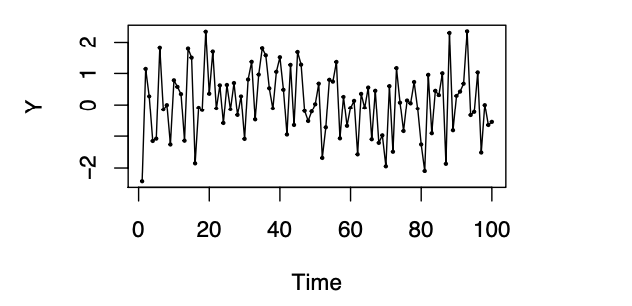
\includegraphics[width=0.75\linewidth]{images/L3-2.png}
                    \caption{A simulated path of a Gaussian white noise process, with \(Y \sim \mathcal{N}(0,1) \)}
                    \label{fig:L3-2}
                \end{figure}

                We will present more example in the next lectures, including Markov processes, ARMA models, Hidden Markov processes, dynamic linear models\ldots\! Let’s first see some important general notions.

\newpage
        \section{Summaries}

            For a random variable $X$, we are used to providing summaries such as the mean (i.e.\ the expected value $E(X)$) and the variance $V(X)$. For a random vector $(X,Y)$, we would provide measures of dependence, such as the covariance
            \begin{equation}
                \mathrm{Cov}(X,Y) \;=\; E\bigl((X - E(X))(Y - E(Y))\bigr),
            \end{equation}
            and the correlation coefficient
            \begin{equation}
                \rho \;=\; \frac{\mathrm{Cov}(X,Y)}{\sqrt{V(X)\,V(Y)}}.
            \end{equation}

            We want to provide similar summaries for time series. A main difference is that, for a time series $(Y_t)$, the mean and the variance, as well as other relevant measures, will generally depend on time. More precisely, let us define the following notions.

            \begin{definition}[Mean function]
                The mean function of $(Y_t)$ is the function
                \[
                \mu:\; t \;\mapsto\; \mu(t) \;=\; F(Y_t), 
                \quad t = 1, 2, \ldots.
                \]
                In the Gaussian white noise example above, the mean function is constant: $\mu(t) = \mu$ for any $t$. In general, however, $F(Y_t)$ varies with $t$ and, roughly speaking, the mean function expresses the expected path over time.
            \end{definition}

            \begin{definition}[Variance function]
                The variance function of $(Y_t)$ is the function
                \[
                \sigma^2:\; t \;\mapsto\; \sigma^2(t) \;=\; V(Y_t), \quad t = 1, 2, \ldots.
                \]
            \end{definition}

            \begin{definition}[Autocovariance function]
                The autocovariance function of $(Y_t)$ is the function
                \[
                \gamma:\; (t_1, t_2) \;\mapsto\; \gamma(t_1, t_2) \;=\; \mathrm{Cov}\bigl(Y_{t_1}, Y_{t_2}\bigr),\quad t_1, t_2 = 1, 2, \ldots,
                \]
                with $\gamma(t, t) = \sigma^2(t)$.
            \end{definition}

            \begin{definition}[Autocorrelation function]
                The autocorrelation function of $(Y_t)$ is the function 
                \[
                \rho:\; (t_1, t_2) \;\mapsto\;  \rho\bigl(t_1, t_2\bigr)  \;=\; \frac{\mathrm{Cov}\bigl(Y_{t_1}, Y_{t_2}\bigr)}{\sqrt{\sigma^2(t_1)\,\sigma^2(t_2)}}, \quad t_1, t_2 = 1, 2, \ldots.
                \]
            \end{definition}

            The autocovariance function and the autocorrelation function inherit several  properties from the properties of the covariance and the correlation coefficient  for random vectors. See Chatfield, Chapter~3.

\newpage
        \section{Stationarity}

            Many statistical models, such as popular ARMA processes, assume that the time series under study is \textit{stationary}.

            \begin{definition}[Strict stationarity]\label{def:strict_stat}
            A time series $(Y_t)$ is \emph{strictly stationary} if the joint distribution of 
            \[
            (Y_t, Y_{t+1}, \ldots, Y_{t+k})
            \]
            does not depend on $t$, for any $k = 1, 2, \ldots$. 
            \end{definition}
            
            This implies that
            
            \[
            (Y_{t_1}, \ldots, Y_{t_k}) \,\overset{d}{=} \,(Y_{t_1 + h}, \ldots, Y_{t_k + h}),
            \]
            
            \noindent for any choice of times $(t_1, \ldots, t_k)$ and any lag $h$, where $\overset{d}{=}$ means equality in distribution. In particular, the marginal distribution of $Y_t$ does not depend on $t$, i.e.,
            
            \[
            Y_1 \,\overset{d}{=} \,Y_2 \,\overset{d}{=} \,\dots \,\overset{d}{=} \,Y_t \,\overset{d}{=} \,\dots.
            \]
            
            \noindent If $E(Y_t)$ and $E(Y_t\,Y_{t+h})$ exist and are finite, this implies that the mean function and variance function are constant over time, namely
            
            \[
            \mu(t) = \mu \quad\text{and}\quad \sigma^2(t) = \sigma^2.
            \]
            
            Moreover, the bivariate distribution of $(Y_t, Y_{t+h})$ does not depend on $t$. thus,
            \[
            (Y_1, Y_{1+h}) \,\overset{d}{=} \,(Y_2, Y_{2+h})  \,\overset{d}{=} \,\dots \,\overset{d}{=} \,(Y_t,Y_{t+h}) \,\overset{d}{=} \,\dots.
            \]
            Consequently, the autocovariance $\gamma(t,t+h)$, which depends on the distribution of $(Y_t, Y_{t+h})$, does not depend on $t$ but only on the lag $h$.
            
            \begin{definition}[Stationarity]\label{def:stationarity}
            A time series $(Y_t)$ is \emph{stationary} (or, more precisely, \emph{second-order stationary}) if $E(Y_t)$ and $E(Y_t Y_{t+h})$ exist and do not depend on $t$, for every lag $h = 1, 2, \ldots$.
            \end{definition}
    
            \begin{figure}[h]
                    \centering
                    \begin{tikzpicture}[scale=1.0,>=stealth]
                    
                        \draw[->] (0,0) -- (7,0) node[right]{time};
                        \draw[->] (0,0) -- (0,5);
                    
                        \foreach \x in {1,2,3,4,5,6}
                        \draw (\x,0) -- (\x,0.1);
                      
                    
                        \draw[dashed] (0,2.5) -- (6,2.5);
                        
                        \draw[domain=-2:2,samples=100,smooth]
                            plot
                            ({2 - 0.4*exp(-(\x*\x)/0.5)}, % x-coord
                            {2.5 + \x});                   % y-coord
                    
                        \draw[dashed] (2,0) -- (2,5);
                    
                        \draw[domain=-1.7:2,samples=100,smooth]
                            plot
                            ({5 - 2*exp(-(\x*\x)/0.5)}, % x-coord
                            {2.5 + \x});                   % y-coord
                    
                            \draw[dashed] (5,0) -- (5,5);
                    
                        \node at (5.9,2.3) {\(\mu(t) = \mu\)};
                    
                    \end{tikzpicture}
                    \caption{Stationarity does not imply strict stationarity. For example, the \(Y_t\) may have the same mean, but the marginal distributions (of \(Y_1\) and of \(Y_t\), in the plot) are different.}
                    \label{fig:L3-3}
                \end{figure}

\newpage

                In other words, this means that

                \begin{align}
                    \mu(t) = \mu & \quad \text{the mean function is constant}, \\
                    \sigma^2(t) = \ \sigma^2 & \quad \text{the variance function is constant}, \\
                    \gamma(t, t + h) = \ \tilde{\gamma}(h) & \quad\text{the autocovariance function only depends on the lag } h.
                \end{align} 
                
                Clearly, a strictly stationary time series with finite second moments is also stationary. However, the reverse is not true. See another beautiful hand-made picture in Figure~3.
                
                The two notions are equivalent for a \emph{Gaussian} time series, that is, for any $(t_1, \ldots, t_k)$, the joint density is Gaussian
                \[
                \begin{bmatrix}
                Y_{t_1} \\
                \vdots \\
                Y_{t_k}
                \end{bmatrix}
                \sim 
                \mathcal{N}_k \!\left(
                \begin{bmatrix}
                \mu(t_1) \\
                \vdots \\
                \mu(t_k)
                \end{bmatrix},
                \begin{bmatrix}
                \sigma^2(t_1) & \gamma(t_1, t_2) & \cdots & \gamma(t_1, t_k) \\
                \gamma(t_2, t_1) & \sigma^2(t_2) & \cdots & \gamma(t_2, t_k) \\
                \vdots          & \vdots          & \ddots & \vdots          \\
                \gamma(t_k, t_1)& \gamma(t_k, t_2)& \cdots & \sigma^2(t_k)
                \end{bmatrix}
                \right)
                \]
                
                You can find an overview of main properties of multivariate Gaussian distributions in the Appendix of the textbook
                Petrone, Petris, Campagnoli,\emph{ \textit{Dynamic Linear Models}}, Springer 2009.
                
                \begin{example}[Gaussian white noise]
                    If $Y_t^{\,\mathrm{i.i.d.}} \sim \mathcal{N}(\mu,\sigma^2)$, then
                    \[
                    \mu(t) = \mu, 
                    \quad
                    \gamma(t,t) = \sigma^2,
                    \quad
                    \gamma(t,t') = 0 \quad (t \neq t').
                    \]
                \end{example}
                
                In the next lecture, we will introduce random walks and Markov processes, that will be very important tools for our developments.


    \chapter{Random walks}

            \begin{mybox}{BlueGreen}{\textbf{References}}

                lecture notes on BBoard and Feller, ``\emph{Introduciton to Probability Theory}'' Chapter 14 (page 360 of the PDF in Desktop \(\rightarrow\) Bocconi \(\rightarrow\) ESS Y1S2 \(\rightarrow\) 20236 Books)
                
            \end{mybox}

            \begin{mybox}{Dandelion}{\textbf{From the previous lecture}}
                In statistical time series analysis, we regard a time series as a stochastic process (i.e. a sequence of random variables or random vectors indexed by physical time \((Y_t)_{t\geq1}\)).

                \noindent Statistical model: \((Y_t)_{t\geq1} \sim \mathbb{P} \)

                To choose a statistical model, it is enough to specify the finite-dimensional distribution (i.e. the univariate, bivariate, ..., multivariate distribution) with some consistency conditions
            \end{mybox}

        \section{Simple Random Walk}

            Statisticians usually have this \textit{explain} step. Suppose we have this data:

            \begin{figure}[h]
                \centering
                \begin{tikzpicture}
                    \draw[->] (0,0) -- (7,0) node[right]{time};
                    \draw[->] (0,0) -- (0,5);
                    
                    \foreach \x in {1,2,3,4,5,6}
                    \draw (\x,0) -- (\x,0.1);                    
                \end{tikzpicture}
                \caption{Graphical representation of an investment}
                \label{fig:L4-1}
            \end{figure}

            \begin{mybox}{BlueGreen}{}

                Leo Breiman, \emph{"The Two Cultures"}, Statistical Science, 2001
                
            \end{mybox}

            \begin{equation}
                y_o>0, \text{ at each step} \begin{cases}
                    +1 \quad \text{with probability } p \\
                    -1 \quad \text{with probability } 1-p
                \end{cases}
            \end{equation}

            \[
            Z \sim \begin{cases}
                -1 \quad \text{with probability } 1-p \\
                +1 \quad \text{with probability } p 
            \end{cases}
            \]

            Take as starting condition \( Y_0 = y_0\), and define the successive steps as \(Y_1= y_0 + Z_1\) and \(Y_2 = Y_1 + Z_2 = y_0 + Z_1 +Z_2\).

            \begin{figure}[h]
                \centering
                \begin{tikzpicture}
                    \draw[->] (0,0) -- (7,0) node[right]{time};
                    \draw[->] (0,0) -- (0,5);
                    
                    \foreach \x in {1,2,3,4,5,6}
                    \draw (\x,0) -- (\x,0.1);                    
                \end{tikzpicture}
                \caption{Graphical representation of an investment}
                \label{fig:L4-2}
            \end{figure}

            \begin{definition}[Simple random walk]
                We define \((Y_t)\) as a simple random walk.
            \end{definition}

            \begin{remark}
                \(Y_t\) depends on the past only through the very last value.
            \end{remark}

                Now let's consider the case where \(Z_t\) is not necessarily binary as in the previous case, but it is instead described as follows:

            \begin{definition}[General random walk]
                Take \((Y_t)_{t \geq 1}\) starting at \(y_0\).
                Now define:
                \begin{equation}
                    Z_t \sim \text{with } E(Z_t)=\mu, \quad V(Z_t)=\sigma^2, \quad \text{usually gaussian}
                \end{equation}

                We get to the law of motion:

                \begin{equation}
                    Y_t = Y_{t-1} + Z_t = y_0 + \sum^t_{i=1} Z_i
                \end{equation}
            \end{definition}

            \begin{proposition}
                Is \((Y_t)\) stationary? In order to verify this, we need to check whether 
                \begin{enumerate}[label=\roman*.]
                    \item \( \mu(t) = \mu \quad \Rightarrow \quad \mu(t)=E(Y_t)= E(\underbrace{y_0}_{y_0=0} + \sum^t_{i=1} \overbrace{Z_i}^{E(Z_i)=0}) = \sum^t_{i=1}E(Z_i)=0 \)
                    \item \(\sigma^2(t)=\sigma^2 \quad \Rightarrow \quad \)
                    \item It is superfluous to check for the 3rd condition
                \end{enumerate}
            \end{proposition}

            \begin{example}
                Assume a model that predicts a price based on the following law of motion:\footnote{A classical assumption for perfect financial markets}
                \[
                \underset{\log(\text{price})=\log P_t}{Y_t}= Y_{t-1} + Z_t
                \]

                Now define the returns as
                \[
                \text{returns}: \frac{P_t}{P_{t-1}} \quad \text{log returns}: Y_t-Y_{t-1}= Z_t
                \]

                This shows that returns are i.i.d. distributed in a random fashion, i.e. \((Z_t)_{t \geq 1} \sim \ldots \quad \text{stationary}\)
                
            \end{example}

            \begin{example}[Random walk with noise]

                \begin{equation}
                    \begin{cases}
                        \overset{\text{Ideal log price}_{t}}{X_t}= X_{t-1} + Z_t \quad \text{latent noise} \\
                        Y_t = X_t + \varepsilon_t, \quad \varepsilon \overset{\text{i.i.d.}}{\sim} N(0,\sigma^2_{\varepsilon})
                    \end{cases}
                \end{equation}
                
            \end{example}
            

    \chapter{Markov processes}

            \begin{mybox}{BlueGreen}{\textbf{References}}

                lecture notes on BBoard
                
            \end{mybox}

        \section{Markov chains}

                First of all, some notation:

                \[
                \underset{Y_t \in \{ 1,\cdots,k \} }{(Y_t)}_{t \geq 1} \sim \mathbb{P} \quad 
                \]

                We also ought to define:  

                \begin{align}
                    (\text{i.i.d.}) \Rightarrow &  \mathbb{P} (y_1, \ldots, y_n) = \mathbb{P} (Y_1 = y_1 \cdots Y_n = y_n) = \mathbb{P} (y_1) \cdot \ldots \cdot \mathbb{P} (y_n) = \prod^n_{i=1} p(y_i) \\
                    (\text{general case}) \Rightarrow & \mathbb{P} (y_1, \ldots, y_n) = \cdots = \mathbb{P} (y_1) \cdot \mathbb{P} (y_2 | y_1) \cdot \ldots \cdot \mathbb{P} (y_n | y_{n-1}) = \prod^n_{i=1} p(y_i | y_{i-1}) \\
                    (\text{Markov}) \Rightarrow & \mathbb{P} (y_1, \ldots, y_n) 
                \end{align}

            \begin{definition}[Markov chain]
                
            \end{definition}

            From the definition it follows that a finite dimensional distribution can be written as in here (see eq.5)

            \noindent To specify the probability law \(\mathbb{P}\) of a Markov chain \((Y_t), \ Y_t \in \{ 1,2, \ldots, k \}\) it is enough to give:
                \begin{enumerate}[label=\roman*.]
                    \item \textbf{Initial probabilities}:
                        \[
                        p_0 
                        \]
                    \item \textbf{Transition probabilities}:
                \end{enumerate}

    \chapter{Inference for Markov chains}

            \begin{mybox}{BlueGreen}{\textbf{References}}

                lecture notes on BBoard
                
            \end{mybox}

    \chapter{Stationary time series: ARMA models I}

            \begin{mybox}{BlueGreen}{\textbf{References}}

                A basic reference is Chatfield (2004), Ch.3 (pp 39-49), Ch. 4, Ch 5, section 5.2.4
                
            \end{mybox}

    \chapter{Stationary time series: ARMA models II}

        \section{Quick overview of ARMA models}

    Classic models presented in a conurs in time series analysis deal with \textbf{stationary processes}.

    Autoregressive and 

    \subsection{For Stationary Time Series}

        \[
        (T_t)_{t \geq 1} \text{ is stationary} 
        \]

        Stationarity is defined and characterized by:
        
            \begin{itemize}
                \item \textbf{Mean} $\mu(t) = \E(T_t) = \mu $
                \item \textbf{Variance} $\sigma(t) = \Var(T_t) =  \sigma^2$
                \item \textbf{Autocovariance} $\gamma(t, t+h) = Cov(Y_t, Y_{t+h}) = \tilde{\gamma}(h)$
                \item \textbf{Autocorrelation} $\rho(t, t+h) = \frac{\gamma(t, t+h)}{\sigma(t)\sigma(t+h)} = \tilde{\rho}(h)$
            \end{itemize}

        Both autocovariance and autocorrelation are functions of the lag $h$.

        If the series \((Y_t)_{t \geq 1}\) is stationary, then the mean, variance, autocovariance and autocorrelation are constant over time and they can be calculated. In fact, we can see that:
            
            \begin{itemize}
                \item Sample mean: \(\hat{\mu} = \frac{\sum_{t=}^{T} Y_t}{T} = \bar{Y}\)
                \item Sample variance: \(\hat{\sigma}^2 = \frac{\sum_{t=1}^{T} (Y_t - \bar{Y})^2}{T-1}\)\footnote{By dividing by $T-1$ instead of $T$, we actually get the "corrected" sample variance.}
                \item Sample autocovariance at lag \(h\): \(\hat{\gamma}(h) = \frac{\sum_{t=1}^{T-h} (Y_t - \bar{Y})(Y_{t+h} - \bar{Y})}{T-h}\)
                \item Sample autocorrelation at lag \(h\): \(\hat{\rho}(h) = \frac{\hat{Cov}(Y_t, Y_{t+h})}{\sqrt{\hat{Var}(Y_t)\hat{Var}(Y_{t+h})}} = \frac{\hat{\gamma}(h)}{\hat{\gamma}(0)}\)
            \end{itemize}

        Plot the estimated \textbf{autocorrelogram} to see if the series is stationary.

        \begin{figure}
            \begin{tikzpicture}
                \draw[->] (0,0) -- (10,0) node[right] {$h$};
                \draw[->] (0,0) -- (0,5) node[above] {$\hat{\rho}(h)$};
                \draw[scale=1,domain=0:10,smooth,variable=\x,blue] plot ({\x},{4*exp(-\x/2)});
            \end{tikzpicture}
        \end{figure}

        The estimated autocorrelation function should be approximately close to the autocorrelation sample for large sample size.

        \begin{proposition}
            Informally speaking, one can expect that:

            Correlogram \(\approx\) True autocorrelation function
        \end{proposition}

    \subsection{For Non-Stationary Time Series}

        In this case, we cannot use the same properties as the moments we used before now depend on time (i.e.\(\mu(t) = E(Y_t) = \mu_t\)).

        \subsubsection{Replicates}

            In some applications (e.g. a financial market with multiple assets prices as time series) we have "replicates" (a random sample) of time series.
            
            INSERISCI GRAFICO

            And we can use

            \begin{equation}
                \bar{Y}_t = \frac{\sum_{i=1}^{n}Y_{i,t}}{n}
            \end{equation}

            to estimate the mean of the time series \( \mu_t = E(Y_t) \).

            However, in many applications we do not have access to replicates.

            As we will see, these models introduce a temporal dependence for the \(\mu_t\), \(\sigma_t\) and \(\gamma_t\), so that observations at times different from \(t\) can still give "indirect" information on \(mu_t\), and can thus be used for estimating it.

\section{ARMA(p,q) Models for Stationary Time Series}

    INSERT THE GRAPH OF THE REALISATION OF A TIME SERIES.

    Suppose we have time series data that can be modeled as the realisation of a stationary time series \((Y_t)_{t \geq 1}\).

    \textit{But what model should we use?} \textbf{ARMA(p,q)} models are a good starting point. One of the reasons why they are attractive is because the order \(p,q\) can be estimated from the data, and it can then be understood from the ACF.

    \subsection{AR(1) autoregressive process of order 1}

        An AR(1) is presented as the (stationary and causal) solution of a finite difference stochastic equation, with \(t \in (-\infty, +\infty)\):

        \begin{equation}
            Y_t = \alpha T_{t-1} + \varepsilon_t 
        \end{equation}

        where \(\varepsilon_t\) is a white noise process with mean 0 and variance \(\sigma^2\), i.e. \(\varepsilon_t \sim N(0, \sigma^2)\).

        A solution of the equation is a proces \(Y_t\) that satisfies the equation for all \(t\). In general, the solution is not unique, but we can impose some conditions to make it unique.
        Namely, if we restrict to stationary solutions, then either there exist no solutions or there exists a unique solution, depending on the value of \(\alpha\).

        \begin{example}[\(\alpha =1\)]
            To define the AR(1) process, we need to specify:
            \[
            \alpha = 1, \quad Y_t = T_{t-1} + \varepsilon_t, \quad \varepsilon_t \sim N(0, \sigma^2)
            \]
            In this case, the model just specified is a random walk, and does not hence admit a stationary solution.
        \end{example}

        \begin{example}[\(|\alpha| < 1\)]
            If instead we consider a model specified as:
            \[
            \alpha \in (-1, 1), \quad Y_t = \alpha Y_{t-1} + \varepsilon_t, \quad \varepsilon_t \sim N(0, \sigma^2)
            \]
            then the model admits a stationary solution, and it is:
            \[
            Y_t = \sum_{j=0}^{\infty} \alpha^j \varepsilon_{t-j} \quad \text{which is an MA}(\infty) \text{ process}
            \]
        \end{example}

        \begin{remark}
            Please note that the above solution is finite if and only if the series converges, which is only possible if \(\alpha \in (-1, 1)\).
        \end{remark}

        GUARDA NOTE SUL GRUPPO: Lemma 1.29 AR(p)

        Let the absolute value of \(\alpha\) be strictly less than 1, then there exists a stationary solution given by \( Y_t = \sum_{j=0}^{\infty} \alpha^j \varepsilon_{t-j} \).

        \begin{equation}
            \forall \alpha \in (-1,1) \quad  \exists ! Y_t = \sum_{j=0}^{\infty} \alpha^j \varepsilon_{t-j}
        \end{equation}



        Let us check that this solution is stationary:

        \begin{itemize}
            \item \textbf{Mean}: 
            \[
            \mu(t) = \E(Y_t) = \E\left(\sum_{j=0}^{\infty} \alpha^j \varepsilon_{t-j}\right) = \sum_{j=0}^{\infty} \alpha^j \E(\varepsilon_{t-j}) = 0
            \]
            \item \textbf{Variance}:
            \[
            \sigma^2(t) = \Var(Y_t) = \Var\left(\sum_{j=0}^{\infty} \alpha^j \varepsilon_{t-j}\right) = \sum_{j=0}^{\infty} \alpha^{2j} \Var(\varepsilon_{t-j}) = \sigma^2 \sum_{j=0}^{\infty} \alpha^{2j} = \frac{\sigma^2}{1-\alpha^2} = \sigma^2 \cdot \frac{1}{1-\alpha^2} = \sigma^2_Y
            \]
            \item \textbf{Autocovariance}:
            \[
            \gamma(t, t+h) = \Cov(Y_t, Y_{t+h}) = E(Y_t, Y_{t+h}) - \underbrace{E(Y_t)}_{0} \overbrace{E(Y_{t+h})}^{0} = \E\left(\sum_{j=0}^{\infty} \alpha^j \varepsilon_{t-j}, \sum_{j=0}^{\infty} \alpha^j \varepsilon_{t+h-j}\right) = E(\alpha^0 \varepsilon_t + \alpha^1 \varepsilon_{t-1} + \ldots, \alpha^h \varepsilon_{t} + \alpha^{h+1} \varepsilon_{t-1} + \ldots) = \alpha^h \frac{\sigma^2}{1-\alpha^2} = \alpha^h \sigma^2_Y
            \]
        \end{itemize}

        Given that all the moments are constant over time (the result on the right do not depend on \(t\)), we can say that the solution is stationary.

        \begin{example}[Do it yourself!]
            Plot the \textit{acf} of an AR(1) process with:
            \begin{enumerate}
                \item \(\alpha = 0.8\)
                \item \(\alpha = -0.8\)
                \item \(\alpha = 2\)
                \item \(\alpha = 0.2\)
            \end{enumerate}
        \end{example}

            The \textit{acf} is \(\rho(g) = \frac{\gamma(h)}{\gamma(0)} = \frac{\alpha^h \cdot \sigma^2_Y}{\sigma^2_Y} = \alpha^h\).
            Thus, the functions can be plotted as

            \begin{tikzpicture}
                \begin{axis}[
                    title={Autocorrelation},
                    xlabel={Lag},
                    ylabel={ACF},
                    xmin=-0.5, xmax=40.5,  % adjust as needed
                    ymin=-1,    ymax=1,    % adjust as needed
                    grid=major,
                    width=12cm, height=6cm,
                ]
                
                % ------------------------------------------------------------------
                % 1) Confidence band (replace 0.2 with the actual +/- CI you need):
                % ------------------------------------------------------------------
                \addplot [name path=upper, draw=none] coordinates {(0, 0.2) (40, 0.2)};
                \addplot [name path=lower, draw=none] coordinates {(0, -0.2) (40, -0.2)};
                
                \addplot [blue!20] fill between[of=upper and lower];
                
                % ------------------------------------------------------------------
                % 2) Horizontal zero line:
                % ------------------------------------------------------------------
                \addplot [domain=-0.5:40.5, color=black, thick] {0};
                
                % ------------------------------------------------------------------
                % 3) Autocorrelation spikes (dummy data):
                %    Replace with your real ACF data, either inline or via \addplot table{...}
                % ------------------------------------------------------------------
                \addplot [
                    ycomb,
                    mark=*,
                    color=blue,
                ] coordinates {
                    (0, 1.0)
                    (1, 0.8)
                    (2, 0.64)
                    (3, 0.512)
                    (4, 0.4096)
                    (5, 0.32768)
                    (6, 0.262144)
                    (7, 0.2097152)
                    (8, 0.16777216)
                    (9, 0.134217728)
                    (10, 0.1073741824)
                    (11, 0.08589934592)
                    (12, 0.068719476736)
                    % ... up to (40, someValue)
                };
                
                \end{axis}
                \end{tikzpicture}

            Oftentimes, it is not sufficient to look at the autocorrelation function: we need to look at the \textit{partial autocorrelation function}.

        \subsubsection{Partial Autocorrelation Function}

            \begin{definition}[Partial Autocorrelation Function]
                For gaussian processes (and ARMA models are indeed Gaussian):
                \begin{equation}
                    \phi:h \mapsto \phi(h) = Corr(Y_t, Y_{t+h} | Y_{t+1}, \ldots, Y_{t+h-1})
                \end{equation}
            \end{definition}

            \begin{example}
                For an autoregressive process of order 1, AR(1), we have:
                \begin{align}
                    \phi(0) &= 1 \\
                    \phi(1) &= Corr(Y_t, Y_{t-1}) \neq 0 \\
                    \phi(2) &= Corr(Y_t, Y_{t-2} | Y_{t-1}) = 0 \\
                    \vdots & \\
                    \phi(h) &= 0 \quad \forall h > 1
                \end{align}
            \end{example}

    \subsection{AR(p) autoregressive process of order p}

        \subsubsection{Partial Autocorrelation Function}

            \begin{definition}[Partial Autocorrelation Function]
            
            \end{definition}

    \subsection{MA(q) moving average process of order q}

            \begin{example}
            
            \end{example}

\section{ARMA(p,q) Process}

    \subsection{Fitting and ARMA model: the Box-Jenkins approach}

        \subsubsection{Step 0: is this series stationary}

        \subsubsection{Step 1: model specification}

        \subsubsection{Step 2: model estimation}

        \subsubsection{Step 3: model diagnostics}
        
    \part[Inference for Non-Stationary Time Series]{Inference for Non-Stationary Time Series: State-Space Models}

    \chapter{Hidden Markov Models (HMMs)}

            \begin{mybox}{BlueGreen}{\textbf{References}}

                lecture notes on BB
                
            \end{mybox}

    \chapter*{LAB 2}

\part{State-Space Models (SSMs) for Time Series Analysis}

    \chapter[State-space models]{State-space models: Definition and main properties}

        Definition and main properties.
        Examples:
        HMMs as state-space models (This is done in class, look at your notes)
        Dynamic Linear Models (DLMs)
        Examples of non-linear, non-Gaussian state-space models (stochastic volatility models).

        \begin{mybox}{BlueGreen}{\textbf{References}}

            Petris, Petrone \& Campagnoli (2009), Chapter 2.
            
        \end{mybox}

    \chapter{Applying SSMs}

        Applying DLMs with known parameters:
        Model specification.
        Filtering, smoothing and forecasting.
        --The simplest non-trivial example: random walk plus noise. (a) Static case; it requires notions of Bayesian inference.

        \begin{mybox}{BlueGreen}{\textbf{References}}

            Petris, Petrone \& Campagnoli (2009), Chapter 2.
            
        \end{mybox}

    \chapter{Basic notions of Bayesian inference I}

        \begin{mybox}{BlueGreen}{\textbf{References}}

            Petris, Petrone \& Campagnoli (2009), Chapter 1. The Gaussian example, with known variance, is on page 7
            
        \end{mybox}

    \chapter{Basic notions of Bayesian inference II}

%-------------------------------------------------

    \chapter[Kalman filter for DLMs I]{Kalman filter for DLMs with known parameters I}

        \begin{mybox}{BlueGreen}{\textbf{References}}

            Petris, Petrone \& Campagnoli (2009), Chapter 2.
            Behavior for large t (random walk plus noise : reference: textbook on DLMs, Ch 3
            
        \end{mybox}

        Back to the basic example: random walk plus noise. (b) Dynamic case: Filtering (with details on computations)

        Kalmam filter for general DLMs

        Example: linear growth model.

    \chapter[Kalman filter for DLMs II]{Kalman filter for DLMs with known parameters II}

    \chapter*{LAB 3: DLMs with R}

%-------------------------------------------------

    \chapter{Smoothing, forecasting, model checking I}

        \begin{mybox}{BlueGreen}{\textbf{References}}

            Petris, Petrone \& Campagnoli (2009), Chapter 2.
            
        \end{mybox}

        Smoothing in DLMs: Kalman smoother

        Forecasting.

        The innovation process. Model checking.

    \chapter{Smoothing, forecasting, model checking II}

%-------------------------------------------------

    \chapter{DLMs with unknown parameters: MLE}

        \begin{mybox}{BlueGreen}{\textbf{References}}

            Petris, Petrone \& Campagnoli (2009), Chapter 4, section 4.1.
            
        \end{mybox}

        Likelihood function for DLMs. MLE and asymptotic standard errors.

    \chapter*{LAB 4: MLE for DLMs with R}

%-------------------------------------------------

    \chapter{Modeling time series with DLMs: examples I}

        \begin{mybox}{BlueGreen}{\textbf{References}}

            Petris, Petrone \& Campagnoli (2009), Chapter 3; only the general idea for local seasonal factors DLMs; no Fourier-based DLMs.
            
        \end{mybox}

        Combining DLMs components

        Basic structural models:

        DLMs for trend.

        DLMs for seasonality (no details)

    \chapter{Modeling time series with DLMs: examples II}

        \begin{mybox}{BlueGreen}{\textbf{References}}

            Petris, Petrone \& Campagnoli (2009), Chapter 3.
            
        \end{mybox}

%-------------------------------------------------

    \chapter{DLMs for spatio-temporal data I}

        \begin{mybox}{BlueGreen}{\textbf{References}}

            No infos
            
        \end{mybox}

    \chapter{DLMs for spatio-temporal data II}

%-------------------------------------------------

    \chapter[Bayesian inference for DLMs]{Bayesian inference for DLMs with unknown parameters}

        \begin{mybox}{BlueGreen}{\textbf{References}}

            Petris, Petrone \& Campagnoli (2009), Chapter 4.
            
        \end{mybox}

        Basic notions.
    
        Markov Chain Monte Carlo (MCMC; only aims and general idea)

        \begin{mybox}{BlueGreen}{\textbf{References for MCMC}}

            Petris, Petrone \& Campagnoli (2009), Chapter 4.
            
        \end{mybox}

\end{document}
